\section{Research Project Timeline}
\label{app:timeline}

\begin{figure}[htbp]
  \centering
  \resizebox{\linewidth}{!}{% Two-semester timeline (weeks) with milestones; simple Gantt drawn in TikZ
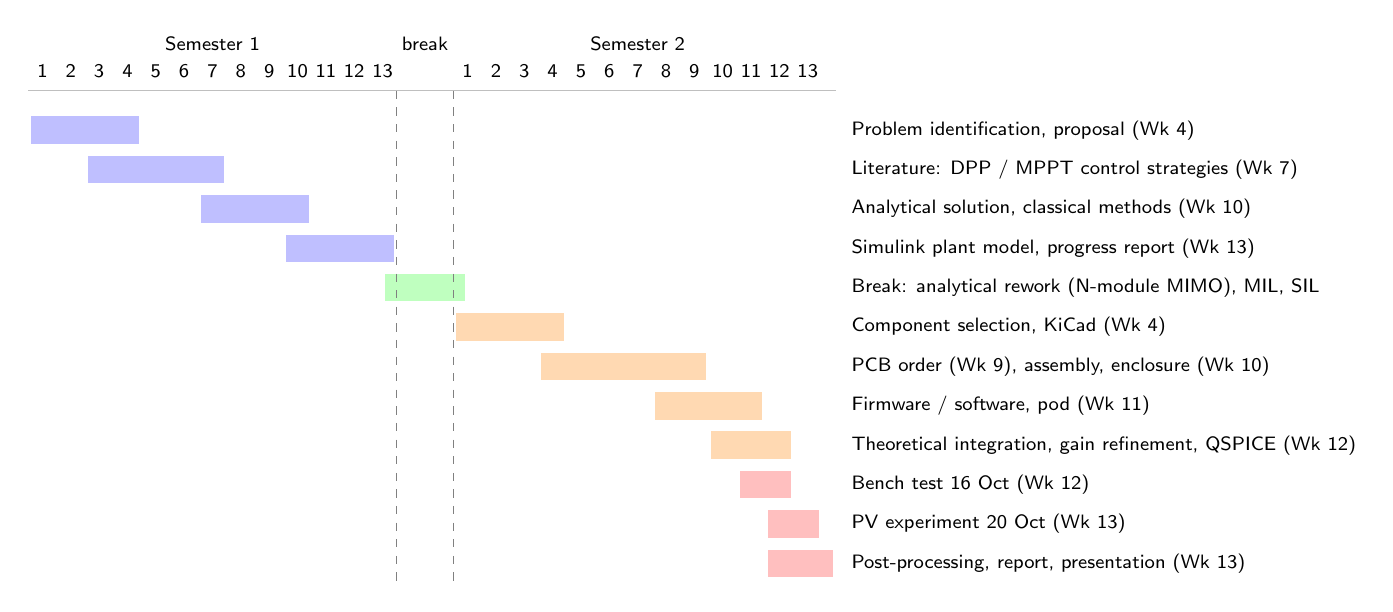
\begin{tikzpicture}[x=0.36cm,y=0.5cm,font=\sffamily\scriptsize]
  % axes: semester 1 weeks 1-13, break, semester 2 weeks 1-13
  \foreach \w in {1,...,13}{\node at (\w,0.5) {\w};}
  \node at (7,1.2) {Semester 1};
  \foreach \w in {1,...,13}{\node at (\w+15,0.5) {\w};}
  \node at (22,1.2) {Semester 2};
  \node at (14.5,1.2) {break};
  \draw[gray!50] (0.5,0) -- (29,0);
  \newcommand{\gbar}[5]{\fill[#5] (#1-0.4,-#3*1.0-0.35) rectangle (#2+0.4,-#3*1.0+0.35); \node[anchor=west] at (29.2,-#3) {#4};}
  \gbar{1}{4}{1}{Problem identification, proposal (Wk 4)}{blue!25}
  \gbar{3}{7}{2}{Literature: DPP / MPPT control strategies (Wk 7)}{blue!25}
  \gbar{7}{10}{3}{Analytical solution, classical methods (Wk 10)}{blue!25}
  \gbar{10}{13}{4}{Simulink plant model, progress report (Wk 13)}{blue!25}
  \gbar{13.5}{15.5}{5}{Break: analytical rework (N-module MIMO), MIL, SIL}{green!25}
  \gbar{16}{19}{6}{Component selection, KiCad (Wk 4)}{orange!30}
  \gbar{19}{24}{7}{PCB order (Wk 9), assembly, enclosure (Wk 10)}{orange!30}
  \gbar{23}{26}{8}{Firmware / software, pod (Wk 11)}{orange!30}
  \gbar{25}{27}{9}{Theoretical integration, gain refinement, QSPICE (Wk 12)}{orange!30}
  \gbar{26}{27}{10}{Bench test 16 Oct (Wk 12)}{red!25}
  \gbar{27}{28}{11}{PV experiment 20 Oct (Wk 13)}{red!25}
  \gbar{27}{28.5}{12}{Post-processing, report, presentation (Wk 13)}{red!25}
  \draw[dashed,gray] (13.5,0) -- (13.5,-12.5);
  \draw[dashed,gray] (15.5,0) -- (15.5,-12.5);
\end{tikzpicture}
}
  \caption{Project timeline across the two semesters (teaching weeks) with the milestone week of each phase.}
  \label{fig:timeline}
\end{figure}

\begin{table}[htbp]\centering\small
\caption{Development phases and their V-model counterpart.}
\label{tab:phases}
\begin{tabular}{c l l l}
\toprule
Phase & Pipeline & V-model & Primary artefact\\
\midrule
0 & Background research & Concept of operations & proposal, literature review\\
1 & Analytical solution & System requirements & \code{nstring.py}, notebooks, \cref{app:analytical}\\
2 & Model-in-the-loop & High-level design & \code{power\_shuffler\_sim.slx} (4 modules)\\
3 & Component selection & Detailed design & KiCad Version 0 PCB, BOM\\
4 & Firmware / software & Development & \code{6\_RTOS} (C), \code{7\_Pi} (Python, Docker)\\
5 & Software-in-the-loop & Unit verification & C Caller blocks, golden replay\\
6 & QSPICE integration & Subsystem verification & QSPICE integrated model + control DLL\\
7 & Bench test & System verification & 16 Oct 2026, 10 windows (\cref{tab:T1})\\
8 & Solar test, partial shade & System validation & 20 Oct 2026, 11 windows (\cref{tab:T1})\\
9 & Post-processing / synthesis & Acceptance & \code{8\_Results/analysis} (\code{make all})\\
\bottomrule
\end{tabular}
\end{table}

\begin{table}[htbp]\centering\small
\caption{Milestones and progress achieved (proposal $\rightarrow$ progress report $\rightarrow$ delivery).}
\label{tab:timeline}
\begin{tabular}{l l l p{6.2cm}}
\toprule
Semester & Week & Milestone & Progress / change\\
\midrule
1 & 4 & Problem identification, proposal & Research question, objectives, risk register, Gantt (34 weeks)\\
1 & 7 & Existing DPP / MPPT control strategies & Literature review (Appendix A of the proposal), gap statement\\
1 & 10 & Analytical solution using classical methods & Single-shuffler averaged model, equilibrium, linearisation, cascaded PI; marginal stability found\\
1 & 13 & Simulink plant model & 4-module PV string, P--V validation, inner current loop attempt (instability under shade)\\
Break & -- & Analytical rework, MIL, SIL & MIMO reformulation (LQR + integral, then decoupling PI), $N$-module string model, MIL 7-test suite, SIL C core + golden replay\\
2 & 4 & Component selection & STM32G474 Nucleo, TMCS1126, INA239, Raspberry Pi 4B; KiCad Version 0\\
2 & 9 & PCB order & PCBWay board + stencil, components, reflow\\
2 & 10 & Enclosure development & Enclosure, heatsink, pod wiring (IR, LCD, LED, DS18B20)\\
2 & 11 & Firmware / software & Bare-metal C application, control core, telemetry contract, Pi stack (Docker InfluxDB + Grafana)\\
2 & 12 & Theoretical integration / gain refinement & QSPICE integrated model with the control DLL; gain sets per $\fsw$; $R_{sw}$ identified\\
2 & 12 & Bench test & 16 Oct 2026: 200/300/400\,kHz, open and closed loop (\cref{tab:T1})\\
2 & 13 & PV experiment & 20 Oct 2026: 3 $\times$ KAUSSP80 in the carpark, $k=0.1\ldots0.8$\\
2 & 13 & Post-processing & Results pipeline (\code{make all}), REPORT.md, this report, presentation\\
\bottomrule
\end{tabular}
\end{table}

Three things changed from the proposal. The first PCB moved from Semester~1 Week~10 into Semester~2 (progress report, Appendix~A), and the planned Version~1 and Version~2 boards collapsed into a single Version~0 board, which meant compromising on PCB revisions and features. String MPPT integration was deferred, because the electronic load performs it. Interim milestones were reviewed weekly with the supervisor.
